\section{Results}
\label{sec:results}

\begin{figure*}[ht]
\begin{tabular}{ccc}
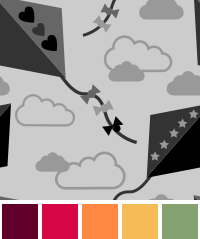
\includegraphics[width=.15\linewidth]{figs/permutationTemplatePalette} & 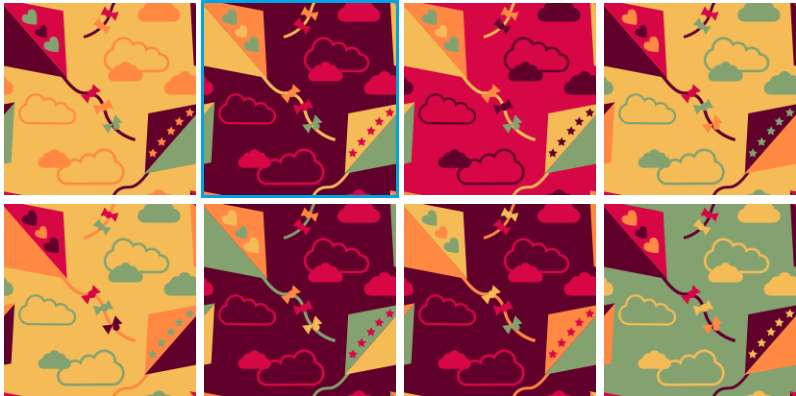
\includegraphics[width=.4\linewidth]{figs/permutationBest8} & 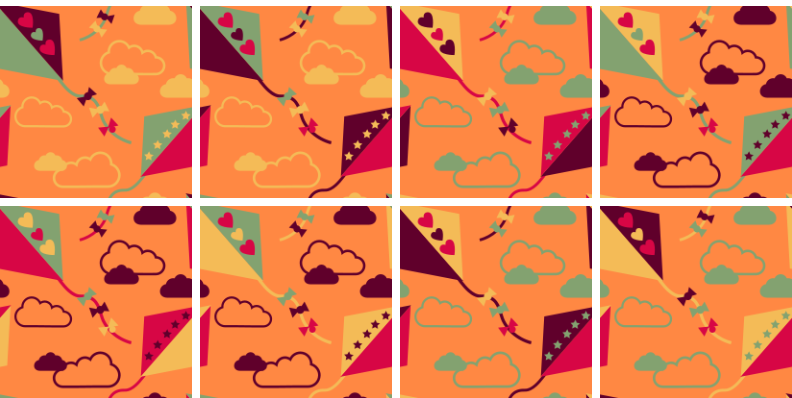
\includegraphics[width=.4\linewidth]{figs/permutationWorst8} %& 
\includegraphics[width=.12\linewidth]{figs/permutationArtist}
  \\
\textbf{(a)} Input Pattern & \textbf{(b)} Highest-scoring assignments & \textbf{(c)} Lowest-scoring assignments %& \textbf{(d)} Artist assignment
\\
\end{tabular}

\caption{Given a segmented image and corresponding palette as input, we use our color model to compute the likelihood of each possible assignment of the palette to the image regions. \textbf{(b)} and \textbf{(c)} show the top-eight and bottom-eight assignments, respectively. The assignment provided by the artist received the second-highest score and is highlighted in blue.}
\label{fig:permutation}
\vspace{-1.0em}
\end{figure*}

\begin{figure}[ht]
\begin{tabular}{cc}

\includegraphics[width=.22\columnwidth]{figs/guidedSearch0Original}&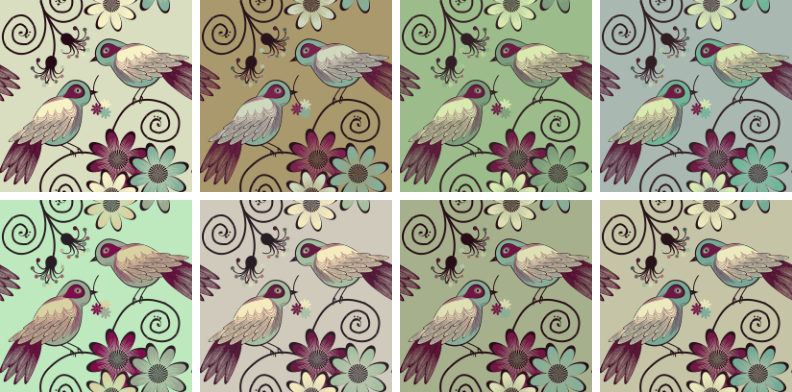
\includegraphics[width=.7\columnwidth]{figs/guidedSearch0MMR}\vspace{0.5em}\\
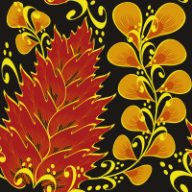
\includegraphics[width=.22\columnwidth]{figs/guidedSearch1Original}&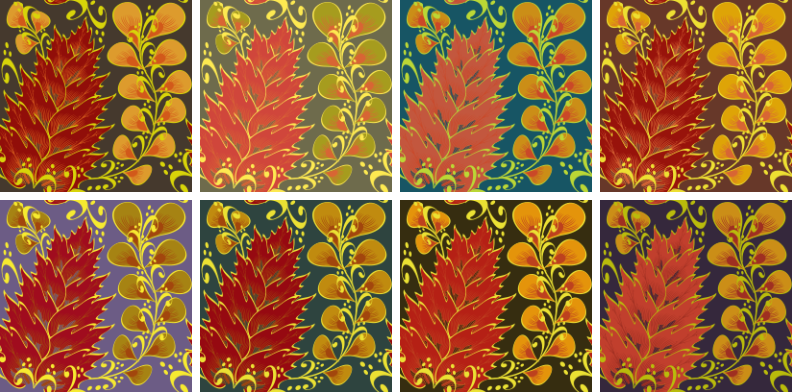
\includegraphics[width=.7\columnwidth]{figs/guidedSearch1MMR}\\
Suggested colors&Highest-scoring assignments\\
\end{tabular}

\caption{An artist provides an initial color assignment and asks for patterns that are similar. We incorporate this request by adding an additional factor to our model, showing eight MMR-diversified samples for the images on the left.}
\label{fig:nearbySuggestions}
\vspace{-1.0em}
\end{figure}

Lots of pictures

Quantitative results from reconstruction experiments, etc.

Performance figures? (training time, inference time, etc.)